%*****************************************
\chapter{Fundamental Skills}\label{ch01:fundamental_skills}
%*****************************************

Microsoft® Excel® is a tool that can be used in virtually all careers and is valuable in both professional and personal settings. Whether you need to keep track of medications in inventory for a hospital or create a financial plan for your retirement, Excel enables you to do these activities efficiently and accurately. This chapter introduces the fundamental skills necessary to get you started in using Excel. You will find that just a few skills can make you very productive in a short period of time.

\section{Overview of Microsoft Excel}

\begin{center}
	\begin{objbox}{Learning Objectives}
		\begin{itemize}
			\setlength{\itemsep}{0pt}
			\setlength{\parskip}{0pt}
			\setlength{\parsep}{0pt}
			
			\item Examine the value of using Excel to make decisions.
			\item Learn how to start Excel.
			\item Become familiar with the Excel workbook.
			\item Understand how to navigate worksheets.
			\item Examine the Excel Ribbon.
			\item Examine the right-click menu options.
			\item Learn how to save workbooks.
			\item Examine the Status Bar.
			\item Become familiar with the features in the Excel Help window.
			
		\end{itemize}
	\end{objbox}
\end{center}

Microsoft® Office contains a variety of tools that help people accomplish many personal and professional objectives. Microsoft Excel is perhaps the most versatile and widely used of all the Office applications. No matter which career path you choose, you will likely need to use Excel to accomplish your professional objectives, some of which may occur daily. This chapter provides an overview of the Excel application along with an orientation for accessing the commands and features of an Excel workbook.

\subsection{Making Decisions With Excel}

Taking a very simple view, Excel is a tool that allows you to enter quantitative data into an electronic spreadsheet to apply one or many mathematical computations. These computations ultimately convert that quantitative data into information. The information produced in Excel can be used to make decisions in both professional and personal contexts. For example, employees can use Excel to determine how much inventory to buy for a clothing retailer, how much medication to administer to a patient, or how much money to spend to stay within a budget. With respect to personal decisions, you can use Excel to determine how much money you can spend on a house, how much you can spend on car lease payments, or how much you need to save to reach your retirement goals. We will demonstrate how you can use Excel to make these decisions and many more throughout this text.

Figure \ref{01:fig01} shows a completed Excel worksheet that will be constructed in this chapter. The information shown in this worksheet is top-line sales data for a hypothetical merchandise retail company. The worksheet data can help this retailer determine the number of salespeople needed for each month, how much inventory is needed to satisfy sales, and what types of products should be purchased.

\begin{figure}[H]
	\centering
	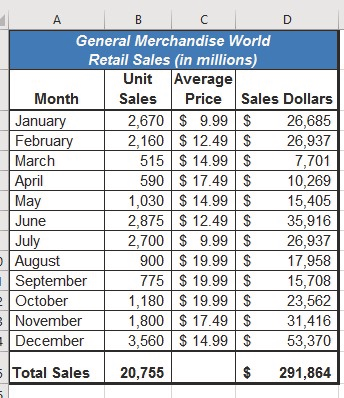
\includegraphics[width=\maxwidth{.95\linewidth}]{gfx/ch01_fig01}
	\caption{Example of an Excel Worksheet}
	\label{01:fig01}
\end{figure}

\subsection{Starting Excel}

\begin{enumerate}
	\item Locate Excel on your computer.
	\item Click Microsoft Excel to launch the Excel application and present you with workbook options.
	\item Click the first option; “Blank Workbook”.
\end{enumerate}

\subsection{The Excel Workbook}

Once Excel is started, a blank workbook will open on your screen. A workbook is an Excel file that contains one or more worksheets (sometimes referred to as spreadsheets). Excel will assign a file name to the workbook, such as \textbf{Book1}, \textbf{Book2}, \textbf{Book3}, and so on, depending on how many new workbooks are opened. Figure \ref{01:fig02} shows a blank workbook after starting Excel. Take some time to familiarize yourself with this screen. Your screen may be slightly different based on the version being used.

\begin{figure}[H]
	\centering
	\includegraphics[width=\maxwidth{.95\linewidth}]{gfx/Ch01_fig02}
	\caption{Blank Workbook}
	\label{01:fig02}
\end{figure}

Your workbook should already be maximized (or shown at full size) once Excel is started, as shown in Figure \ref{01:fig02}. However, if your screen looks like Figure \ref{01:fig03} after starting Excel, you should click the Maximize button, as shown in the figure.

\begin{figure}[H]
	\centering
	\includegraphics[width=\maxwidth{.95\linewidth}]{gfx/Ch01_fig03}
	\caption{Restored Worksheet}
	\label{01:fig03}
\end{figure}

\subsection{Navigating Worksheets}

Data are entered and managed in an Excel worksheet. The worksheet contains several rectangles called cells for entering numeric and nonnumeric data. Each cell in an Excel worksheet contains an address, which is defined by a column letter followed by a row number. For example, the cell that is currently activated in Figure \ref{01:fig03} is \textsf{A1}. This would be referred to as cell location \textsf{A1} or cell reference \textsf{A1}. The following steps explain how you can navigate in an Excel worksheet:

\begin{itemize}
	\item Place your mouse pointer over cell \textsf{D5} and left click.
	\item Check to make sure column letter D and row number 5 are highlighted, as shown in Figure \ref{01:fig04}.
\end{itemize}

\begin{figure}[H]
	\centering
	\includegraphics[width=\maxwidth{.95\linewidth}]{gfx/Ch01_fig04}
	\caption{Activating a Cell Location}
	\label{01:fig04}
\end{figure}

\begin{enumerate}
	\item Move the mouse pointer to cell \textsf{A1}.
	\item Click and hold the left mouse button and drag the mouse pointer back to cell \textsf{D5}.
	\item Release the left mouse button. You should see several cells highlighted, as shown in Figure \ref{01:fig05}.
\end{enumerate}

This is referred to as a cell range and is documented as follows: \textsf{A1:D5}. Any two cell locations separated by a colon are known as a cell range. The first cell is the top left corner of the range, and the second cell is the lower right corner of the range.

\begin{figure}[H]
	\centering
	\includegraphics[width=\maxwidth{.95\linewidth}]{gfx/Ch01_fig05}
	\caption{Highlighting a Range of Cells}
	\label{01:fig05}
\end{figure}

\begin{enumerate}
	\item At the bottom of the screen, you'll see worksheets. Depending on your version of Excel, you will see either three as displayed in Figure \ref{01:fig05} or just one. If you only have one sheet, click the ``Insert Worksheet'' to add a worksheet. Depending on your version, you instead may have a \textsf{+} sign; a click on the \textsf{+} adds an additional worksheet as well. This is how you open or add a worksheet within a workbook. Add another worksheet so that you now have three sheets displaying here.
	\item Click the \textit{Sheet1} worksheet tab at the bottom of the worksheet to return to the worksheet shown in Figure \ref{01:fig05}.
\end{enumerate}

\begin{center}
	\begin{shtcutbox}{Keyboard Shortcuts}
		\textbf{Basic Worksheet Navigation}
		\\
		\begin{itemize}
			\setlength{\itemsep}{0pt}
			\setlength{\parskip}{0pt}
			\setlength{\parsep}{0pt}

			\item Use the arrow keys on your keyboard to activate cells on the worksheet.
			\item Hold the SHIFT key and press the arrow keys on your keyboard to highlight a range of cells in a worksheet.
			\item Hold the CTRL key while pressing the PAGE DOWN or PAGE UP keys to open other worksheets in a workbook.

		\end{itemize}
	\end{shtcutbox}
\end{center}

\subsection{The Excel Ribbon}

Excel's features and commands are found in the Ribbon, which is the upper area of the Excel screen that contains several tabs running across the top. Each tab provides access to a different set of Excel commands. Figure \ref{01:fig06} shows the commands available in the Home tab of the Ribbon. Table \ref{01:tab01}, ``Command Overview for Each Tab of the Ribbon,'' provides an overview of the commands that are found in each tab of the Ribbon.

\begin{figure}[H]
	\centering
	\includegraphics[width=\maxwidth{.95\linewidth}]{gfx/Ch01_fig06}
	\caption{Home Tab of the Ribbon}
	\label{01:fig06}
\end{figure}

\begin{table}[H]
	\centering
	\definecolor{ltgray}{gray}{0.95} % this is a light gray
	\rowcolors{1}{}{ltgray} % zebra striping background
	\begin{tabularx}{0.95\linewidth}{
			p{0.15\linewidth}
			p{0.85\linewidth}}
		\toprule
		\textbf{Tab} & \textbf{Description} \\
		\midrule

		File & Also known as the Backstage view of the Excel workbook. Contains all commands for opening, closing, saving, and creating new Excel workbooks. Includes print commands, document properties, e-mailing options, and help features. The default settings and options are also found in this tab.\\

		Home & Contains the most frequently used Excel commands. Formatting commands are found in this tab along with commands for cutting, copying, pasting, and for inserting and deleting rows and columns.\\

		Insert & Used to insert objects such as charts, pictures, shapes, PivotTables, Internet links, symbols, or text boxes.\\
		
		Page Layout & Contains commands used to prepare a worksheet for printing. Also includes commands used to show and print the gridlines on a worksheet.\\
		
		Formulas & Includes commands for adding mathematical functions to a worksheet. Also contains tools for auditing mathematical formulas.\\

		Data & Used when working with external data sources such as Microsoft® Access®, text files, or the Internet. Also contains sorting commands and access to scenario tools.\\
		
		Review & Includes Spelling and Track Changes features. Also contains protection features to password protect worksheets or workbooks.\\
		
		View & Used to adjust the visual appearance of a workbook. Common commands include the Zoom and Page Layout view.\\
		
		\bottomrule
	\end{tabularx}
	\caption{Command Overview for Ribbon Tabs}
	\label{01:tab01}
\end{table}

The Ribbon shown in Figure \ref{01:fig06} is full, or maximized. The benefit of having a full Ribbon is that the commands are always visible while you are developing a worksheet. However, depending on the screen dimensions of your computer, you may find that the Ribbon takes up too much vertical space on your worksheet. If this is the case, you can minimize the Ribbon by clicking the button shown in Figure \ref{01:fig06}. When minimized, the Ribbon will show only the tabs and not the command buttons. When you click on a tab, the command buttons will appear until you select a command or click anywhere on your worksheet.

\begin{center}
	\begin{shtcutbox}{Keyboard Shortcuts}
		\textbf{Minimizing or Maximizing the Ribbon}
		\\
		\begin{itemize}
			\setlength{\itemsep}{0pt}
			\setlength{\parskip}{0pt}
			\setlength{\parsep}{0pt}
			
			\item Hold down the CTRL key and press the F1 key.
			\item Hold down the CTRL key and press the F1 key again to maximize the Ribbon.
			
		\end{itemize}
	\end{shtcutbox}
\end{center}

\subsection{Quick Access Toolbar and Right-Click Menu}

The Quick Access Toolbar is found at the upper left side of the Excel screen above the Ribbon, as shown in Figure \ref{01:fig07}. This area provides access to the most frequently used commands, such as Save and Undo. You also can customize the Quick Access Toolbar by adding commands that you use on a regular basis. By placing these commands in the Quick Access Toolbar, you do not have to navigate through the Ribbon to find them. To customize the Quick Access Toolbar, click the down arrow as shown in Figure \ref{01:fig07}. This will open a menu of commands that you can add to the Quick Access Toolbar. If you do not see the command you are looking for on the list, select the More Commands option.

\begin{figure}[H]
	\centering
	\includegraphics[width=\maxwidth{.95\linewidth}]{gfx/Ch01_fig07}
	\caption{Customizing the Quick Access Toolbar}
	\label{01:fig07}
\end{figure}

In addition to the Ribbon and Quick Access Toolbar, you can also access commands by right clicking anywhere on the worksheet. Figure 1.8 shows an example of the commands available in the right-click menu.

\begin{figure}[H]
	\centering
	\includegraphics[width=\maxwidth{.95\linewidth}]{gfx/Ch01_fig08}
	\caption{Right-Click Menu}
	\label{01:fig08}
\end{figure}

\subsection{The File Tab}

The File tab is also known as the Backstage view of the workbook. It contains a variety of features and commands related to the workbook that is currently open, new workbooks, or workbooks stored in other locations on your computer or network. Figure \ref{01:fig09} shows the options available in the File tab or Backstage view. To leave the Backstage view and return to the worksheet, click the arrow in the upper left-hand corner as shown below.

\begin{figure}[H]
	\centering
	\includegraphics[width=\maxwidth{.95\linewidth}]{gfx/Ch01_fig09}
	\caption{File Tab or Backstage View of a Workbook}
	\label{01:fig09}
\end{figure}

Included in the File tab are the default settings for the Excel application that can be accessed and modified by clicking the Options button. Figure \ref{01:fig10} shows the Excel Options window, which gives you access to settings such as the default font style, font size, and the number of worksheets that appear in new workbooks.

\begin{figure}[H]
	\centering
	\includegraphics[width=\maxwidth{.95\linewidth}]{gfx/Ch01_fig10}
	\caption{Excel Options Window}
	\label{01:fig10}
\end{figure}

\subsection{Saving Workbooks (Save As)}

Once you create a new workbook, you will need to change the file name and choose a location on your computer or network to save that file. It is important to remember where you save this workbook on your computer or network as you will be using this file in the Section 1.2 “Entering, Editing, and Managing Data” to construct the workbook shown in Figure \ref{01:fig01}. The process of saving can be different with different versions of Excel. Please be sure you follow the steps for the version of Excel you are using. The following steps explain how to save a new workbook and assign it a file name.

\subsubsection{Saving Workbooks in Excel 2013}

\begin{enumerate}
	\item If you have not done so already, open a blank workbook in Excel.
	\item When saving your workbook for the \textit{first} time, click the File tab.
	\item Click the Save As button in the upper left side of the Backstage view window. This will open the Save As dialog box, as shown in Figure \ref{01:fig11}.
	\item Click in the File Name box at the bottom of the Save As dialog box and use the BACKSPACE key to remove the current default name of the workbook.
	\item Type the file name: \textbf{CH1 GMW Sales Data}.
	\item Click the Desktop button on the left side of the Save As dialog box if you wish to save this file on your desktop. If you want to save this workbook in a different location, such as a USB drive, select your preferred location.
	\item Click the Save button on the lower right side of the Save As dialog box.
	\item As you continue to work on your workbook, you will want to Save frequently by click either the Save button on the Home ribbon or by selecting the Save option from the File menu.
\end{enumerate}

\begin{figure}[H]
	\centering
	\includegraphics[width=\maxwidth{.95\linewidth}]{gfx/Ch01_fig11}
	\caption{Save As Dialog Box in Excel 2013}
	\label{01:fig11}
\end{figure}

\subsubsection{Saving Workbooks in Excel 2016}

\begin{itemize}
	\item If you have not done so already, open a blank workbook in Excel.
	\item Click the File tab and then the Save As button in the left side of the Backstage view window. This will open the Save As dialog box.
	\item Determine a location for saving on your computer by clicking Browse on the left side to open the Save As dialog box as illustrated in Figure \ref{01:fig12}.
	\item Click in the File Name box near the bottom of the Save As dialog box. Type the new file name: \textbf{CH1 GMW Sales Data}
	\item Review the settings in the screen for correctness and click the Save button.
\end{itemize}

\begin{figure}[H]
	\centering
	\includegraphics[width=\maxwidth{.95\linewidth}]{gfx/Ch01_fig12}
	\caption{Save As Dialog in 2016}
	\label{01:fig12}
\end{figure}

\begin{center}
	\begin{shtcutbox}{Keyboard Shortcuts}
		\textbf{Save As}
		\\
		\begin{itemize}
			\setlength{\itemsep}{0pt}
			\setlength{\parskip}{0pt}
			\setlength{\parsep}{0pt}
			
			\item Press the F12 key and use the tab and arrow keys to navigate around the Save As dialog box. Use the ENTER key to make a selection.
			\item Or press the ALT key on your keyboard. You will see letters and numbers, called Key Tips, appear on the Ribbon. Press the F key on your keyboard for the File tab and then the A key. This will open the Save As dialog box.
			
		\end{itemize}
	\end{shtcutbox}
\end{center}

\begin{center}
	\begin{sklbox}{Skill Refresher}
		\textbf{Saving Workbooks (Save As)}
		\\
		\begin{itemize}
			\setlength{\itemsep}{0pt}
			\setlength{\parskip}{0pt}
			\setlength{\parsep}{0pt}
			
			\item Click the File tab on the Ribbon.
			\item Click the Save As option.
			\item Select a location on your PC.
			\item Click in the File name box and type a new file name if needed.
			\item Click the down arrow next to the ``Save as type'' box and select the appropriate file type if needed.
			\item Click the Save button.
		
		\end{itemize}
	\end{sklbox}
\end{center}

\subsection{The Status Bar}

The Status Bar is located below the worksheet tabs on the Excel screen (see Figure 1.13). It displays a variety of information, such as the status of certain keys on your keyboard (e.g., CAPS LOCK), the available views for a workbook, the magnification of the screen, and mathematical functions that can be performed when data are highlighted on a worksheet. You can customize the Status Bar as follows:

\begin{enumerate}
	\item 1. Place the mouse pointer over any area of the Status Bar and right click to display the ``Customize Status Bar'' list of options (see Figure 1.13).
	\item Select the Caps Lock option from the menu (see Figure \ref{01:fig13}).
	\item Press the CAPS LOCK key on your keyboard. You will see the Caps Lock indicator on the lower right side of the Status Bar.
	\item Press the CAPS LOCK on your keyboard again. The indicator on the Status Bar goes away.
\end{enumerate}

\begin{figure}[H]
	\centering
	\includegraphics[width=\maxwidth{.95\linewidth}]{gfx/Ch01_fig13}
	\caption{Customizing the Status Bar}
	\label{01:fig13}
\end{figure}

\subsection{Excel Help}

The Help feature provides extensive information about the Excel application. Although some of this information may be stored on your computer, the Help window will automatically connect to the Internet, if you have a live connection, to provide you with resources that can answer most of your questions. You can open the Excel Help window by clicking the question mark in the upper right area of the screen or ribbon. With newer versions of Excel, use the query box to enter your question and select from helpful option links or select the question mark from the dropdown list to launch Excel Help windows.

\begin{figure}[H]
	\centering
	\includegraphics[width=\maxwidth{.95\linewidth}]{gfx/Ch01_fig14}
	\caption{Excel Help Window}
	\label{01:fig14}
\end{figure}

\begin{center}
	\begin{shtcutbox}{Keyboard Shortcuts}
		\textbf{Excel Help}
		\\
		\begin{itemize}
			\setlength{\itemsep}{0pt}
			\setlength{\parskip}{0pt}
			\setlength{\parsep}{0pt}
			
			\item Press the F1 key on your keyboard.
			
		\end{itemize}
	\end{shtcutbox}
\end{center}


\begin{center}
	\begin{tkwbox}{Key Take-Aways}
		\textbf{Overview}
		\\
		\begin{itemize}
			\setlength{\itemsep}{0pt}
			\setlength{\parskip}{0pt}
			\setlength{\parsep}{0pt}
			
			\item Excel is a powerful tool for processing data for the purposes of making decisions.
			\item You can find Excel commands throughout the tabs in the Ribbon.
			\item You can customize the Quick Access Toolbar by adding commands you frequently use.
			\item You can add or remove the information that is displayed on the Status Bar.
			\item The Help window provides you with extensive information about Excel.
			
		\end{itemize}
	\end{tkwbox}
\end{center}

\section{Entering, Editing, and Managing Data}

\begin{center}
	\begin{objbox}{Learning Objectives}
		\begin{itemize}
			\setlength{\itemsep}{0pt}
			\setlength{\parskip}{0pt}
			\setlength{\parsep}{0pt}
			
			\item Understand how to enter data into a worksheet.
			\item Examine how to edit data in a worksheet.
			\item Examine how Auto Fill is used when entering data.
			\item Understand how to delete data from a worksheet and use the Undo command.
			\item Examine how to adjust column widths and row heights in a worksheet.
			\item Understand how to hide columns and rows in a worksheet.
			\item Examine how to insert columns and rows into a worksheet.
			\item Understand how to delete columns and rows from a worksheet.
			\item Learn how to move data to different locations in a worksheet.

		\end{itemize}
	\end{objbox}
\end{center}

In this section, we will begin the development of the workbook shown in Figure \ref{01:fig01}. The skills covered in this section are typically used in the early stages of developing one or more worksheets in a workbook.

\subsection{Entering Data}

You will begin building the workbook shown in Figure \ref{01:fig01} by manually entering data into the worksheet. The following steps explain how the column headings in Row 2 are typed into the worksheet:

\begin{enumerate}
	\item Click cell location \textsf{A2} on the worksheet.
	\item Type the word \textbf{Month}.
	\item Press the RIGHT ARROW key. This will enter the word into cell \textsf{A2} and activate the next cell to the right.
	\item Type \textbf{Unit Sales} and press the RIGHT ARROW key.
	\item Repeat step 4 for the words \textbf{Average Price} and then again for \textbf{Sales Dollars}.
\end{enumerate}

Figure \ref{01:fig15} shows how your worksheet should appear after you have typed the column headings into Row 2. Notice that the word \textbf{Price} in cell location \textsf{C2} is not visible. This is because the column is too narrow to fit the entry you typed. We will examine formatting techniques to correct this problem in the next section.

\begin{figure}[H]
	\centering
	\includegraphics[width=\maxwidth{.95\linewidth}]{gfx/Ch01_fig15}
	\caption{Entering Column Headings into a Worksheet}
	\label{01:fig15}
\end{figure}

\begin{enumerate}
	\item Click cell location \textsf{B3}.
	\item Type the number \textbf{2670} and press the ENTER key. After you press the ENTER key, cell \textsf{B4} will be activated. Using the ENTER key is an efficient way to enter data vertically down a column.
	\item Enter the following numbers in cells \textsf{B4} through \textsf{B14}: \textbf{2160}, \textbf{515}, \textbf{590}, \textbf{1030}, \textbf{2875}, \textbf{2700}, \textbf{900}, \textbf{775}, \textbf{1180}, \textbf{1800}, and \textbf{3560}.
	\item Click cell location \textsf{C3}.
	\item Type the number \textbf{9.99} and press the ENTER key.
	\item Enter the following numbers in cells \textsf{C4} through \textsf{C14}: \textbf{12.49}, \textbf{14.99}, \textbf{17.49}, \textbf{14.99}, \textbf{12.49}, \textbf{9.99}, \textbf{19.99}, \textbf{19.99}, \textbf{19.99}, \textbf{17.49}, and \textbf{14.99}.
\end{enumerate}

%TODO Start Here


Integrity Check

Column Headings

It is critical to include column headings that accurately describe the data in each column of a worksheet. In
professional environments, you will likely be sharing Excel workbooks with coworkers. Good column headings
reduce the chance of someone misinterpreting the data contained in a worksheet, which could lead to costly errors
depending on your career.




BEGINNING EXCEL 21
7. Activate cell location D3.
8. Type the number 26685 and press the ENTER key.
9. Enter the following numbers in cells D4 through
D14: 26937, 7701, 10269, 15405, 35916, 26937, 17958, 15708, 23562, 31416, and 53370.
10. When finished, check that the data you entered matches Figure 1.16.

EDITING DATA

Data that has been entered in a cell can be changed by double clicking the cell location or using
the Formula Bar. You may have noticed that as you were typing data into a cell location, the data you
typed appeared in the Formula Bar. The Formula Bar can be used for entering data into cells as well
as for editing data that already exists in a cell. The following steps provide an example of entering and
then editing data that has been entered into a cell location:

1. Click cell A15 in the Sheet1 worksheet.
2. Type the abbreviation Tot and press the ENTER key.
3. Click cell A15.
4. Move the mouse pointer up to the Formula Bar. You will see the pointer turn into a cursor.
Move the cursor to the end of the abbreviation Tot and left click.
5. Type the letters al to complete the word Total.




Why?

Avoid Formatting Symbols When Entering Numbers

When typing numbers into an Excel worksheet, it is best to avoid adding any formatting symbols such as dollar signs
and commas. Although Excel allows you to add these symbols while typing numbers, it slows down the process of
entering data. It is more efficient to use Excel’s formatting features to add these symbols to numbers after you type
them into a worksheet.




Integrity Check

Data Entry

It is very important to proofread your worksheet carefully, especially when you have entered numbers. Transposing
numbers when entering data manually into a worksheet is a common error. For example, the number 563 could be
transposed to 536. Such errors can seriously compromise the integrity of your workbook.




22 NOREEN BROWN, BARBARA LAVE, JULIE ROMEY, MARY SCHATZ, DIANE SHINGLEDECKER
Integrity Check

Figure 1.16 shows how your worksheet should appear after entering the data. Check your numbers carefully to
make sure they are accurately entered into the worksheet.




Figure 1.16 Completed Data Entry for Columns B, C, and D




BEGINNING EXCEL 23
6. Click the checkmark to the left of the Formula Bar (see Figure 1.17). This will enter the change
into the cell.




Figure 1.17 Using the Formula Bar to Edit and Enter Data




7. Double click cell A15.
8. Add a space after the word Total and type the word Sales.
9. Press the ENTER key.


Keyboard Shortcuts


Editing Data in a Cell




24 NOREEN BROWN, BARBARA LAVE, JULIE ROMEY, MARY SCHATZ, DIANE SHINGLEDECKER
• Activate the cell that is to be edited and press the F2 key on your keyboard.



AUTO FILL

The Auto Fill feature is a valuable tool when manually entering data into a worksheet. This feature
has many uses, but it is most beneficial when you are entering data in a defined sequence, such as the
numbers 2, 4, 6, 8, and so on, or nonnumeric data such as the days of the week or months of the year.
The following steps demonstrate how Auto Fill can be used to enter the months of the year in Column
A:

1.   Click cell A3 in the Sheet1 worksheet.
2.   Type the word January and press the ENTER key.
3.   Activate cell A3 again.
4.   Move the mouse pointer to the lower right corner of cell A3. You will see a small square in this
corner of the cell; this is called the Fill Handle (See Figure 1.18) When the mouse pointer gets
close to the Fill Handle, the white block plus sign will turn into a black plus sign.




Figure 1.18 Fill Handle


Left click and drag the Fill Handle to cell A14. Notice that the Auto Fill tip box indicates what month
will be placed into each cell (see Figure 1.19). Release the left mouse button when the tip box reads
“December.”

BEGINNING EXCEL 25
Figure 1.19 Using Auto Fill to Enter the Months of the Year


Once you release the left mouse button, all twelve months of the year should appear in the cell range
A3:A14, as shown in Figure 1.20. You will also see the Auto Fill Options button. By clicking this
button, you have several options for inserting data into a group of cells.

26 NOREEN BROWN, BARBARA LAVE, JULIE ROMEY, MARY SCHATZ, DIANE SHINGLEDECKER
Figure 1.20 Auto Fill Options Button


1.   Click the Auto Fill Options button.
2.   Click the Copy Cells option. This will change the months in the range A4:A14 to January.
3.   Click the Auto Fill Options button again.
4.   Click the Fill Months option to return the months of the year to the cell range A4:A14. The Fill
Series option will provide the same result.

DELETING DATA AND THE UNDO COMMAND

There are several methods for removing data from a worksheet, a few of which are demonstrated
BEGINNING EXCEL 27
here. With each method, you use the Undo command. This is a helpful command in the event you
mistakenly remove data from your worksheet. The following steps demonstrate how you can delete
data from a cell or range of cells:

1. Click cell C2 by placing the mouse pointer over the cell and clicking the left mouse button.
2. Press the DELETE key on your keyboard. This removes the contents of the cell.
3. Highlight the range C3:C14 by placing the mouse pointer over cell C3. Then left click and drag
the mouse pointer down to cell C14.
4. Place the mouse pointer over the Fill Handle. You will see the white block plus sign change to a
black plus sign.
5. Click and drag the mouse pointer up to cell C3 (see Figure 1.21). Release the mouse button. The
contents in the range C3:C14 will be removed.




28 NOREEN BROWN, BARBARA LAVE, JULIE ROMEY, MARY SCHATZ, DIANE SHINGLEDECKER
Figure 1.21 Using Auto Fill to Delete Contents of Cell


1. Click the Undo button in the Quick Access Toolbar (see Figure 1.2). This should replace the data
in the range C3:C14.
2. Click the Undo button again. This should replace the data in cell C2.


Keyboard Shortcuts


Undo Command

• Hold down the CTRL key while pressing the letter Z on your keyboard.



BEGINNING EXCEL 29
• Highlight the range C2:C14 by placing the mouse pointer over cell C2. Then left click and drag the mouse
pointer down to cell C14.

• Click the Clear button in the Home tab of the Ribbon, which is next to the Cells group of commands
(see Figure 1.22). This opens a drop-down menu that contains several options for removing or clearing data
from a cell. Notice that you also have options for clearing just the formats in a cell or the hyperlinks in a cell.

• Click the Clear All option. This removes the data in the cell range.

• Click the Undo button. This replaces the data in the range C2:C14.




Figure 1.22 Clear Command Drop-Down Menu


ADJUSTING COLUMNS AND ROWS

There are a few entries in the worksheet that appear cut off. For example, the last letter of the
word September cannot be seen in cell A11. This is because the column is too narrow for this word.
The columns and rows on an Excel worksheet can be adjusted to accommodate the data that is being
entered into a cell. The following steps explain how to adjust the column widths and row heights in a
worksheet:

1. Bring the mouse pointer between Column A and Column B in the Sheet1 worksheet, as shown
in Figure 1.23. You will see the white block plus sign turn into double arrows.

30 NOREEN BROWN, BARBARA LAVE, JULIE ROMEY, MARY SCHATZ, DIANE SHINGLEDECKER
2. Click and drag the column to the right so the entire word September in cell A11 can be seen. As
you drag the column, you will see the column width tip box. This box displays the number of
characters that will fit into the column using the Calibri 11-point font which is the default
setting for font/size.
3. Release the left mouse button.




Figure 1.23 Adjusting Column Widths


You may find that using the click-and-drag method is inefficient if you need to set a specific character
width for one or more columns. Steps 1 through 6 illustrate a second method for adjusting column
widths when using a specific number of characters:

1. Click any cell location in Column A by moving the mouse pointer over a cell location and
clicking the left mouse button. You can highlight cell locations in multiple columns if you are
setting the same character width for more than one column.
2. In the Home tab of the Ribbon, left click the Format button in the Cells group.

BEGINNING EXCEL 31
3. Click the Column Width option from the drop-down menu. This will open the Column Width
dialog box.
4. Type the number 13 and click the OK button on the Column Width dialog box. This will set
Column A to this character width (see Figure 1.24).
5. Once again bring the mouse pointer between Column A and Column B so that the double arrow
pointer displays and then double-click to activate AutoFit. This features adjusts the column
width based on the longest entry in the column.
6. Use the Column Width dialog box (step 6 above) to reset the width to 13.




Figure 1.24 Column Width Dialog Box




Keyboard Shortcuts


Column Width

• Press the ALT key on your keyboard, then press the letters H, O, and W one at a time.



Steps 1 through 4 demonstrate how to adjust row height, which is similar to adjusting column width:

1. Click cell A15 by placing the mouse pointer over the cell and clicking the left mouse button.
2. In the Home tab of the Ribbon, left click the Format button in the Cells group.
3. Click the Row Height option from the drop-down menu. This will open the Row Height dialog
box.

32 NOREEN BROWN, BARBARA LAVE, JULIE ROMEY, MARY SCHATZ, DIANE SHINGLEDECKER
4. Type the number 24 and click the OK button on the Row Height dialog box. This will set Row
15 to a height of 24 points. A point is equivalent to approximately 1/72 of an inch. This
adjustment in row height was made to create space between the totals for this worksheet and the
rest of the data.


Keyboard Shortcuts


Row Height

• Press the ALT key on your keyboard, then press the letters H, O, and H one at a time.



Figure 1.25 shows the appearance of the worksheet after Column A and Row 15 are adjusted.




BEGINNING EXCEL 33
Figure 1.25 GMW Sales Data with Column A and Row 15 Adjusted




Skill Refresher


Adjusting Columns and Rows

1. Activate at least one cell in the row or column you are adjusting.
2. Click the Home tab of the Ribbon.



34 NOREEN BROWN, BARBARA LAVE, JULIE ROMEY, MARY SCHATZ, DIANE SHINGLEDECKER
3. Click the Format button in the Cells group.
4. Click either Row Height or Column Width from the drop-down menu.
5. Enter the Row Height in points or Column Width in characters in the dialog box.
6. Click the OK button.




HIDING COLUMNS AND ROWS

In addition to adjusting the columns and rows on a worksheet, you can also hide columns and rows.
This is a useful technique for enhancing the visual appearance of a worksheet that contains data that is
not necessary to display. These features will be demonstrated using the GMW Sales Data workbook.
However, there is no need to have hidden columns or rows for this worksheet. The use of these skills
here will be for demonstration purposes only.

1. Click cell C1 in the Sheet1 worksheet by placing the mouse pointer over the cell location and
clicking the left mouse button.
2. Click the Format button in the Home tab of the Ribbon.
%3. Place the mouse pointer over the Hide & Unhide option in the drop-down menu. This will open
a submenu of options.
4. Click the Hide Columns option in the submenu of options (see Figure 1.26). This will hide
Column C.




%Figure 1.26 Hide & Unhide Submenu




BEGINNING EXCEL 35
Keyboard Shortcuts


Hiding Columns

• Hold down the CTRL key while pressing the number 0 on your keyboard.



Figure 1.27 shows the workbook with Column C hidden in the Sheet1 worksheet. You can tell a
column is hidden by the missing letter C.




Figure 1.27 Hidden Column


To unhide a column, follow these steps:

1.    Highlight the range B1:D1 by activating cell B1 and clicking and dragging over to cell D1.
2.    Click the Format button in the Home tab of the Ribbon.
%3.    Place the mouse pointer over the Hide & Unhide option in the drop-down menu.
4.    Click the Unhide Columns option in the submenu of options. Column C will now be visible on
the worksheet.

36 NOREEN BROWN, BARBARA LAVE, JULIE ROMEY, MARY SCHATZ, DIANE SHINGLEDECKER
Keyboard Shortcuts


Unhiding Columns

• Highlight cells on either side of the hidden column(s), then hold down the CTRL key and the SHIFT key while
pressing the close parenthesis key ()) on your keyboard.



The following steps demonstrate how to hide rows, which is similar to hiding columns:

1. Click cell A3 in the Sheet1 worksheet by placing the mouse pointer over the cell location and
clicking the left mouse button.
2. Click the Format button in the Home tab of the Ribbon.
%3. Place the mouse pointer over the Hide & Unhide option in the drop-down menu. This will open
a submenu of options.
4. Click the Hide Rows option in the submenu of options. This will hide Row 3.


Keyboard Shortcuts


Hiding Rows

• Hold down the CTRL key while pressing the number 9 key on your keyboard.



To unhide a row, follow these steps:

1.    Highlight the range A2:A4 by activating cell A2 and clicking and dragging over to cell A4.
2.    Click the Format button in the Home tab of the Ribbon.
%3.    Place the mouse pointer over the Hide & Unhide option in the drop-down menu.
4.    Click the Unhide Rows option in the submenu of options. Row 3 will now be visible on the
worksheet.


Keyboard Shortcuts


Unhiding Rows

• Highlight cells above and below the hidden row(s), then hold down the CTRL key and the SHIFT key while
pressing the open parenthesis key (() on your keyboard.




BEGINNING EXCEL 37
Skill Refresher


Hiding Columns and Rows

1. Activate at least one cell in the row(s) or column(s) you are hiding.
2. Click the Home tab of the Ribbon.
3. Click the Format button in the Cells group.
%4. Place the mouse pointer over the Hide & Unhide option.
5. Click either the Hide Rows or Hide Columns option.




Skill Refresher


Unhiding Columns and Rows

1. Highlight the cells above and below the hidden row(s) or to the left and right of the hidden column(s).
2. Click the Home tab of the Ribbon.
3. Click the Format button in the Cells group.
%4. Place the mouse pointer over the Hide & Unhide option.
5. Click either the Unhide Rows or Unhide Columns option.



INSERTING COLUMNS AND ROWS

Using Excel workbooks that have been created by others is a very efficient way to work because it
eliminates the need to create data worksheets from scratch. However, you may find that to accomplish
your goals, you need to add additional columns or rows of data. In this case, you can insert blank
columns or rows into a worksheet. The following steps demonstrate how to do this:

1. Click cell C1 in the Sheet1 worksheet by placing the mouse pointer over the cell location and
clicking the left mouse button.
2. Click the down arrow on the Insert button in the Home tab of the Ribbon (see Figure 1.28).




Integrity Check

Hidden Rows and Columns

In most careers, it is common for professionals to use Excel workbooks that have been designed by a coworker.
Before you use a workbook developed by someone else, always check for hidden rows and columns. You can quickly
see whether a row or column is hidden if a row number or column letter is missing.




38 NOREEN BROWN, BARBARA LAVE, JULIE ROMEY, MARY SCHATZ, DIANE SHINGLEDECKER
Figure 1.28 Insert Button (Down Arrow)




3. Click the Insert Sheet Columns option from the drop-down menu (see Figure 1.29). A blank
column will be inserted to the left of Column C. The contents that were previously in Column C
now appear in Column D. Note that columns are always inserted to the left of the activated cell.




Figure 1.29 Insert Drop-Down Menu




BEGINNING EXCEL 39
Keyboard Shortcuts


Inserting Columns

%◦ Press the ALT key and then the letters H, I, and C one at a time. A column will be inserted to the left of
the activated cell.



4. Click cell A3 in the Sheet1 worksheet by placing the mouse pointer over the cell location and
clicking the left mouse button.
5. Click the down arrow on the Insert button in the Home tab of the Ribbon (see Figure 1.28).
6. Click the Insert Sheet Rows option from the drop-down menu (see Figure 1.29). A blank row
will be inserted above Row 3. The contents that were previously in Row 3 now appear in Row 4.
Note that rows are always inserted above the activated cell.


Keyboard Shortcuts


Inserting Rows

• Press the ALT key and then the letters H, I, and R one at a time. A row will be inserted above the activated
cell.




Skill Refresher


Inserting Columns and Rows

1. Activate the cell to the right of the desired blank column or below the desired blank row.
2. Click the Home tab of the Ribbon.
3. Click the down arrow on the Insert button in the Cells group.
4. Click either the Insert Sheet Columns or Insert Sheet Rows option.



MOVING DATA

Once data are entered into a worksheet, you have the ability to move it to different locations. The
following steps demonstrate how to move data to different locations on a worksheet:

1. Highlight the range D2:D15 by activating cell D2 and clicking and dragging down to cell D15.
2. Bring the mouse pointer to the left edge of cell D2. You will see the white block plus sign change
to cross arrows (see Figure 1.30). This indicates that you can left click and drag the data to a new
location.


40 NOREEN BROWN, BARBARA LAVE, JULIE ROMEY, MARY SCHATZ, DIANE SHINGLEDECKER
Figure 1.30 Moving Data




3. Left Click and drag the mouse pointer to cell C2.
4. Release the left mouse button. The data now appears in Column C.
5. Click the Undo button in the Quick Access Toolbar. This moves the data back to Column D.



DELETING COLUMNS AND ROWS

You may need to delete entire columns or rows of data from a worksheet. This need may arise if
you need to remove either blank columns or rows from a worksheet or columns and rows that
contain data. The methods for removing cell contents were covered earlier and can be used to delete
unwanted data. However, if you do not want a blank row or column in your workbook, you can delete
it using the following steps:

1. Click cell A3 by placing the mouse pointer over the cell location and clicking the left mouse
button.




Integrity Check

Moving Data

Before moving data on a worksheet, make sure you identify all the components that belong with the series you are
moving. For example, if you are moving a column of data, make sure the column heading is included. Also, make sure
all values are highlighted in the column before moving it.




BEGINNING EXCEL 41
2. Click the down arrow on the Delete button in the Cells group in the Home tab of the Ribbon.
3. Click the Delete Sheet Rows option from the drop-down menu (see Figure 1.31). This removes
Row 3 and shifts all the data (below Row 2) in the worksheet up one row.


Keyboard Shortcuts


Deleting Rows

%◦ Press the ALT key and then the letters H, D, and R one at a time. The row with the activated cell will be
deleted.




Figure 1.31 Delete Drop-Down Menu




4. Click cell C1 by placing the mouse pointer over the cell location and clicking the left mouse
button.
5. Click the down arrow on the Delete button in the Cells group in the Home tab of the Ribbon.
6. Click the Delete Sheet Columns option from the drop-down menu (see Figure 1.31). This
removes Column C and shifts all the data in the worksheet (to the right of Column B) over one
column to the left.
7. Save the changes to your workbook by clicking either the Save button on the Home ribbon; or
by selecting the Save option from the File menu.




42 NOREEN BROWN, BARBARA LAVE, JULIE ROMEY, MARY SCHATZ, DIANE SHINGLEDECKER
Keyboard Shortcuts


Deleting Columns

• Press the ALT key and then the letters H, D, and C one at a time. The column with the activated cell will be
deleted.




Skill Refresher


Deleting Columns and Rows

1. Activate any cell in the row or column that is to be deleted.
2. Click the Home tab of the Ribbon.
3. Click the down arrow on the Delete button in the Cells group.
4. Click either the Delete Sheet Columns or the Delete Sheet Rows option.




Key Takeaways


• Column headings should be used in a worksheet and should accurately describe the data contained in each
column.

• Using symbols such as dollar signs when entering numbers into a worksheet can slow down the data entry
process.

• Worksheets must be carefully proofread when data has been manually entered.

• The Undo command is a valuable tool for recovering data that was deleted from a worksheet.

• When using a worksheet that was developed by someone else, look carefully for hidden columns or rows.



ATTRIBUTION

Adapted by Barbara Lave from How to Use Microsoft Excel: The Careers in Practice Series, adapted
by The Saylor Foundation without attribution as requested by the work’s original creator or
licensee, and licensed under CC BY-NC-SA 3.0.




BEGINNING EXCEL 43
1.3 FORMATTING AND DATA ANALYSIS




Learning Objectives


1. Use formatting techniques as introduced in the Excel Spreadsheet Guidelines to enhance the appearance
of a worksheet.
2. Understand how to align data in cell locations.
3. Examine how to enter multiple lines of text in a cell location.
4. Understand how to add borders to a worksheet.
5. Examine how to use the AutoSum feature to calculate totals.
6. Use the Cut, Copy, and Paste commands to manipulate the data on a worksheet.
7. Understand how to move, rename, insert, and delete worksheet tabs.



This section addresses formatting commands that can be used to enhance the visual appearance of
a worksheet. It also provides an introduction to mathematical calculations. The skills introduced in
this section will give you powerful tools for analyzing the data that we have been working with in
this workbook and will highlight how Excel is used to make key decisions in virtually any career.
Additionally, Excel Spreadsheet Guidelines for format and appearance will be introduced as a format
for the course and spreadsheets submitted.

FORMATTING DATA AND CELLS

Enhancing the visual appearance of a worksheet is a critical step in creating a valuable tool for you
or your coworkers when making key decisions. There are accepted professional formatting standards
when spreadsheets contain only currency data. For this course, we will use the following Excel
Guidelines for Formatting. The first figure displays how to use Accounting number format when ALL
figures are currency. Only the first row of data and the totals should be formatted with the Accounting
format. The other data should be formatted with Comma style. There also needs to be a Top Border
above the numbers in the total row. If any of the numbers have cents, you need to format all of the
data with two decimal places.




44 NOREEN BROWN, BARBARA LAVE, JULIE ROMEY, MARY SCHATZ, DIANE SHINGLEDECKER
Figure 1.31a


Often, your Excel spreadsheet will contain values that are both currency and non-currency in nature.
When that is the case, you’ll want to use the guidelines in the following figure:




BEGINNING EXCEL 45
Figure 1.31b


The following steps demonstrate several fundamental formatting skills that will be applied to the
workbook that we are developing for this chapter. Several of these formatting skills are identical to
ones that you may have already used in other Microsoft applications such as Microsoft® Word® or
Microsoft® PowerPoint®.

1. Highlight the range A2:D2 in the Sheet1 worksheet by placing the mouse pointer over cell A2
and left clicking and dragging to cell D2. Click the Bold button in the Font group of commands
in the Home tab of the ribbon.
2. Click the Border button in the Font group of commands in the Home tab of the Ribbon
(see Figure 1.32). Select the Bottom Border option from the list to achieve the goal of a border
on the bottom of row 2 below the column headings.




46 NOREEN BROWN, BARBARA LAVE, JULIE ROMEY, MARY SCHATZ, DIANE SHINGLEDECKER
Figure 1.32 Font Group of Commands




Keyboard Shortcuts


Bold Format

%◦ Hold the CTRL key while pressing the letter B on your keyboard.



3. Highlight the range A15:D15 by placing the mouse pointer over cell A15 and left clicking and
dragging to cell D15.
4. Click the Bold button in the Font group of commands in the Home tab of the Ribbon.
5. Click the Border button in the Font group of commands in the Home tab of the Ribbon
(see Figure 1.32). Select the Top Border option from the list to achieve the goal of a border on
the top of row 15 where totals will eventually display.


Keyboard Shortcuts


Italics Format

%◦ Hold the CTRL key while pressing the letter I on your keyboard.




BEGINNING EXCEL 47
Keyboard Shortcuts


Underline Format

%◦ Hold the CTRL key while pressing the letter U on your keyboard.




1. Highlight the range B3:B14 by placing the mouse pointer over cell B3 and left clicking and
dragging down to cell B14.
2. Click the Comma Style button in the Number group of commands in the Home tab of the
Ribbon. This feature adds a comma as well as two decimal places. (see Figure 1.33).




Why?

Format Column Headings and Totals

Applying formatting enhancements to the column headings and column totals in a worksheet is a very important
technique, especially if you are sharing a workbook with other people. These formatting techniques allow users of
the worksheet to clearly see the column headings that define the data. In addition, the column totals usually contain
the most important data on a worksheet with respect to making decisions, and formatting techniques allow users
to quickly see this information.




48 NOREEN BROWN, BARBARA LAVE, JULIE ROMEY, MARY SCHATZ, DIANE SHINGLEDECKER
Figure 1.33 Number Group of Commands


3. Since the figures in this range do not include cents, click the Decrease Decimal button in the
Number group of commands in the Home tab of the Ribbon two times (see Figure 1.33).
4. The numbers will also be reduced to zero decimal places.
5. Highlight the range C3:C14 by placing the mouse pointer over cell C3 and left clicking and
dragging down to cell C14.
6. Click the Accounting Number Format button in the Number group of commands in the Home
tab of the Ribbon (see Figure 1.33). This will add the US currency symbol and two decimal
places to the values. This format is common when working with pricing data. As discussed
above in the Formatting Data and Cells section, you will want to use Accounting format on all
values in this range since the worksheet contains non-currency as well as currency data.
7. Highlight the range D3:D14 by placing the mouse pointer over cell D3 and left clicking and
dragging down to cell D14.
8. Again, select the Accounting Number Format; this will add the US currency symbol to the
values as well as two decimal places.
9. Click the Decrease Decimal button in the Number group of commands in the Home tab of the
Ribbon.
10. This will add the US currency symbol to the values and reduce the decimal places to zero since
there are no cents in these figures.
11. Highlight the range A1:D1 by placing the mouse pointer over cell A1 and left clicking and
dragging over to cell D1.
12. Click the down arrow next to the Fill Color button in the Font group of commands in the Home
tab of the Ribbon (see Figure 1.34). This will prepare the range for a worksheet title.




BEGINNING EXCEL 49
Figure 1.34 Fill Color Palette




13. Click the Blue, Accent 1, Darker 25% color from the palette (see Figure 1.34). Notice that as you
move the mouse pointer over the color palette, you will see a preview of how the color will
appear in the highlighted cells. Experiment with this feature.
14. Click on A1 and enter the worksheet title: General Merchandise World and click on the check
mark in the formula bar to enter this information.
15. Since the black font is difficult to read on the blue background, you’ll change the font color to be
more visible. Click the down arrow next to the Font Color button in the Font group of
commands in the Home tab of the Ribbon; select White as the font color for this range
(see Figure 1.32).
16. Highlight the range A1:D15 by placing the mouse pointer over cell A1 and left clicking and
dragging down to cell D15.
17. Click the drop-down arrow on the right side of the Font button in the Home tab of the Ribbon;
select Arial as the font for this range. (see Figure 1.32).
18. Notice that as you move the mouse pointer over the font style options, you can see the font
change in the highlighted cells.
19. Expand the column width of Column D to 14 characters.



Figure 1.35 shows how the Sheet1 worksheet should appear after the formatting techniques are
applied.



50 NOREEN BROWN, BARBARA LAVE, JULIE ROMEY, MARY SCHATZ, DIANE SHINGLEDECKER
Figure 1.35 Formatting Techniques Applied




Why?

%Pound Signs (####) Appear in Columns

When a column is too narrow for a long number, Excel will automatically convert the number to a series of pound
%signs (####). In the case of words or text data, Excel will only show the characters that fit in the column. However,
this is not the case with numeric data because it can give the appearance of a number that is much smaller than
what is actually in the cell. To remove the pound signs, increase the width of the column.




BEGINNING EXCEL 51
DATA ALIGNMENT (WRAP TEXT, MERGE CELLS, AND CENTER)

The skills presented in this segment show how data are aligned within cell locations. For example, text
and numbers can be centered in a cell location, left justified, right justified, and so on. In some cases
you may want to stack multiword text entries vertically in a cell instead of expanding the width of a
column. This is referred to as wrapping text. These skills are demonstrated in the following steps:

1. Highlight the range B2:D2 by placing the mouse pointer over cell B2 and left clicking and
dragging over to cell D2.
2. Click the Center button in the Alignment group of commands in the Home tab of the Ribbon
(see Figure 1.36). This will center the column headings in each cell location.




Figure 1.36 Alignment Group in Home Tab




3. Click the Wrap Text button in the Alignment group (see Figure 1.36). The height of Row 2
automatically expands, and the words that were cut off because the columns were too narrow
are now stacked vertically.




52 NOREEN BROWN, BARBARA LAVE, JULIE ROMEY, MARY SCHATZ, DIANE SHINGLEDECKER
Keyboard Shortcuts


Wrap Text

%◦ Press the ALT key and then the letters H and W one at a time.



4. Highlight the range A1:D1 by placing the mouse pointer over cell A1 and left clicking and
dragging over to cell D1.
%5. Click the down arrow on the right side of the Merge & Center button in the Alignment group of
commands in the Home tab of the Ribbon.
%6. Left click the Merge & Center option (see Figure 1.37). This will create one large cell location
running across the top of the data set.


Keyboard Shortcuts


Merge Commands

%• Merge & Center: Press the ALT key and then the letters H, M, and C one at a time.

• Merge Cells: Press the ALT key and then the letters H, M, and M one at a time.

• Unmerge Cells: Press the ALT key and then the letters H, M, and U one at a time.




Why?

Wrap Text

The benefit of using the Wrap Text command is that it significantly reduces the need to expand the column width to
accommodate multiword column headings. The problem with increasing the column width is that you may reduce
the amount of data that can fit on a piece of paper or one screen. This makes it cumbersome to analyze the data in
the worksheet and could increase the time it takes to make a decision.




BEGINNING EXCEL 53
Figure 1.37 Merge Cell Drop-Down Menu




Figure 1.38 shows the Sheet1 worksheet with the data alignment commands applied. The reason for
merging the cells in the range A1:D1 will become apparent in the next segment.




Why?

%Merge & Center

%One of the most common reasons the Merge & Center command is used is to center the title of a worksheet directly
above the columns of data. Once the cells above the column headings are merged, a title can be centered above the
columns of data. It is very difficult to center the title over the columns of data if the cells are not merged.




54 NOREEN BROWN, BARBARA LAVE, JULIE ROMEY, MARY SCHATZ, DIANE SHINGLEDECKER
Figure 1.38 Sheet1 with Data Alignment Features Added




Skill Refresher


Wrap Text

1. Activate the cell or range of cells that contain text data.
2. Click the Home tab of the Ribbon.



BEGINNING EXCEL 55
3. Click the Wrap Text button.




Skill Refresher


Merge Cells

1. Highlight a range of cells that will be merged.
2. Click the Home tab of the Ribbon.
%3. Click the down arrow next to the Merge & Center button.
%4. Select an option from the Merge & Center list.



ENTERING MULTIPLE LINES OF TEXT

In the Sheet1 worksheet, the cells in the range A1:D1 were merged for the purposes of adding a title
to the worksheet. This worksheet will contain both a title and a subtitle. The following steps explain
how you can enter text into a cell and determine where you want the second line of text to begin:

1. Activate cell A1 in the Sheet1 worksheet by placing the mouse pointer over cell A1 and clicking
the left mouse button. Since the cells were merged, clicking cell A1 will automatically activate
the range A1:D1. Position your mouse to the end of the title, directly after the “d” in the word
“World” and double-click to get a cursor (flashing I-beam).
2. Hold down the ALT key and press the ENTER key. This will start a new line of text in this cell
location.
3. Type the text Retail Sales (in millions) and press the ENTER key.
4. Select cell A1. Then click the Italics and Bold buttons in the Font group of commands in the
Home tab of the Ribbon.
5. Increase the height of Row 1 to 30 points. Once the row height is increased, all the text typed
into the cell will be visible (see Figure 1.39).




56 NOREEN BROWN, BARBARA LAVE, JULIE ROMEY, MARY SCHATZ, DIANE SHINGLEDECKER
%Figure 1.39 Title & Subtitle Added to the Worksheet




Skill Refresher


Entering Multiple Lines of Text

1. Activate a cell location.
2. Type the first line of text.
3. Hold down the ALT key and press the ENTER key.
4. Type the second line of text and press the ENTER key.



BORDERS (ADDING LINES TO A WORKSHEET)

In Excel, adding custom lines to a worksheet is known as adding borders. Borders are different from
the grid lines that appear on a worksheet and that define the perimeter of the cell locations. The
Borders command lets you add a variety of line styles to a worksheet that can make reading the
BEGINNING EXCEL 57
worksheet much easier. The following steps illustrate methods for adding preset borders and custom
borders to a worksheet:

1. Click the down arrow to the right of the Borders button in the Font group of commands in the
Home page of the Ribbon to view border options. (see Figure 1.40).Figure 1.40 Borders Drop-
Down Menu




2. Highlight the range A1:D15. Left click the All Borders option from the Borders drop-down
menu (see Figure 1.40). This will add vertical and horizontal lines to the range A1:D15.
3. Highlight the range A2:D2 by placing the mouse pointer over cell A2 and left clicking and
dragging over to cell D2.
4. Click the down arrow to the right of the Borders button.
5. Left click the Thick Bottom Border option from the Borders drop-down menu.
6. Highlight the range A14:D14 and apply a Thick Bottom Border from the drop-down menu. The
thick border will help maintain the Excel Formatting Guidelines.
7. Highlight the range A1:D15.
8. Click the down arrow to the right of the Borders button.
9. Click More Borders… at the bottom of the List.
10. This will open the Format Cells dialog box (see Figure 1.41). You can access all formatting
commands in Excel through this dialog box.
11. In the Style section of the Borders tab, left click the thickest line style (see Figure 1.41).
12. Left click the Outline button in the Presets section (see Figure 1.41).
13. Click the OK button at the bottom of the dialog box (see Figure 1.41).


58 NOREEN BROWN, BARBARA LAVE, JULIE ROMEY, MARY SCHATZ, DIANE SHINGLEDECKER
Figure 1.41 Borders Tab of the Format Cells Dialog Box




BEGINNING EXCEL 59
Figure 1.42 Borders Added to the Sheet1 Worksheet




Skill Refresher


Preset Borders

1. Highlight a range of cells that require borders.
2. Click the Home tab of the Ribbon.
3. Click the down arrow next to the Borders button.
4. Select an option from the preset borders list.

Custom Borders




60 NOREEN BROWN, BARBARA LAVE, JULIE ROMEY, MARY SCHATZ, DIANE SHINGLEDECKER
1. Highlight a range of cells that require borders.
2. Click the Home tab of the Ribbon.
3. Click the down arrow next to the Borders button.
4. Select the More Borders option at the bottom of the options list.
5. Select a line style and line color.
6. Select a placement option.
7. Click the OK button on the dialog box.




AUTOSUM

You will see at the bottom of Figure 1.42 that Row 15 is intended to show the totals for the data
in this worksheet. Applying mathematical computations to a range of cells is accomplished
through functions in Excel. Chapter 2 “Mathematical Computations” will review mathematical
formulas and functions in detail. However, the following steps will demonstrate how you can quickly
sum the values in a column of data using the AutoSum command:

1. Activate cell B15 in the Sheet1 worksheet.
2. Click the Formulas tab of the Ribbon.
3. Click the down arrow below the AutoSum button in the Function Library group of commands
(see Figure 1.43). Note that the AutoSum button can also be found in the Editing group of
commands in the Home tab of the Ribbon.




BEGINNING EXCEL 61
Figure 1.43 AutoSum Drop-Down List




4. Click the Sum option from the AutoSum drop-down menu. The first click will display a flashing
marquee around the range. Click the check mark next to the Formula bar to complete the
function.
5. Excel will provide a total for the values in the Unit Sales column.
6. Activate cell D15. It would not make sense to total the averages in column C so C15 will be left
blank.
7. Repeat steps 3 through 5 to sum the values in the Sales Dollars column (see Figure 1.44).




62 NOREEN BROWN, BARBARA LAVE, JULIE ROMEY, MARY SCHATZ, DIANE SHINGLEDECKER
Figure 1.44 Totals Added to the Sheet1 Worksheet




Skill Refresher


AutoSum

1. Highlight a cell location below or to the right of a range of cells that contain numeric values.
2. Click the Formulas tab of the Ribbon.
3. Click the down arrow below the AutoSum button.
4. Select a mathematical function from the list.



MOVING, RENAMING, INSERTING, AND DELETING WORKSHEETS

The default names for the worksheet tabs at the bottom of workbook are Sheet1, Sheet2, and so on.
However, you can change the worksheet tab names to identify the data you are using in a workbook.
Additionally, you can change the order in which the worksheet tabs appear in the workbook. The
following steps explain how to rename and move the worksheets in a workbook:

1. With the left mouse button, double click the Sheet1 worksheet tab at the bottom of the
workbook (see Figure 1.45). Type the name Sales by Month.
2. Press the ENTER key on your keyboard.

BEGINNING EXCEL 63
3. With the left mouse button, double click the Sheet2 worksheet tab at the bottom of the
workbook.
4. Type the name Unit Sales Rank to prepare the worksheet for future use.
5. Press the ENTER key on your keyboard.




Figure 1.45 Renaming a Worksheet Tab




6. Click the Sheet3 worksheet tab.
7. Click the Home tab of the Ribbon.
8. Click the down arrow on the Delete button in the Cells group of commands.
9. Click the Delete Sheet option from the drop-down list. This removes the unneeded worksheet.
10. Click the Delete button on the Delete warning box (if a warning box appears).
11. Complete the steps above to delete the newly named Unit Sales Rank worksheet since it’s
decided that worksheet is also unnecessary so that you are left with just one worksheet.
12. Save the changes to your workbook by clicking either the Save button on the Home ribbon; or
by selecting the Save option from the File menu.




Integrity Check

Deleting Worksheets

Be very cautious when deleting worksheets that contain data. Once a worksheet is deleted, you cannot use the
Undo command to bring the sheet back. Deleting a worksheet is a permanent command.




64 NOREEN BROWN, BARBARA LAVE, JULIE ROMEY, MARY SCHATZ, DIANE SHINGLEDECKER
Keyboard Shortcuts


Inserting New Worksheets

• Press the SHIFT key and then the F11 key on your keyboard.



Figure 1.46 shows the final appearance of the GMW Sales workbook.




Figure 1.46 Final Appearance of the GMW Sales Workbook




Skill Refresher


Renaming Worksheets

1. Double click the worksheet tab.


BEGINNING EXCEL 65
2. Type the new name.
3. Press the ENTER key.

Moving Worksheets

1. Left click the worksheet tab.
2. Drag it to the desired position.

Deleting Worksheets

1. Open the worksheet to be deleted.
2. Click the Home tab of the Ribbon.
3. Click the down arrow on the Delete button.
4. Select the Delete Sheet option.
5. Click Delete on the warning box.




Key Takeaways


• Formatting skills are critical for creating worksheets that are easy to read and have a professional
appearance.

%• A series of pound signs (####) in a cell location indicates that the column is too narrow to display the
number entered.

• Using the Wrap Text command allows you to stack multiword column headings vertically in a cell location,
reducing the need to expand column widths.

%• Use the Merge & Center command to center the title of a worksheet directly over the columns that contain
data.

• Adding borders or lines will make your worksheet easier to read and helps to separate the data in each
column and row.

• You cannot use the Undo command to bring back a worksheet that has been deleted.



ATTRIBUTION

Adapted by Barbara Lave from How to Use Microsoft Excel: The Careers in Practice Series, adapted
by The Saylor Foundation without attribution as requested by the work’s original creator or
licensee, and licensed under CC BY-NC-SA 3.0.




66 NOREEN BROWN, BARBARA LAVE, JULIE ROMEY, MARY SCHATZ, DIANE SHINGLEDECKER
1.4 PRINTING




Learning Objectives


• Use the Page Layout tab to prepare a worksheet for printing.

• Add headers and footers to a printed worksheet.

• Examine how to print worksheets and workbooks.



Once you have completed a workbook, it is good practice to select the appropriate settings for
printing. These settings are in the Page Layout tab of the Ribbon and discussed in this section of the
chapter.

PAGE SETUP

Before you can properly print the worksheets in a workbook, you must establish appropriate settings.
The following steps explain several of the commands in the Page Layout tab of the Ribbon used to
prepare a worksheet for printing:

1. Open the CH1 GMW Sales workbook, if it is not already open.
2. Click the Page Layout tab of the Ribbon.
3. Click the Margins button in the Page Setup group of commands. This will open a drop-down
list of options for setting the margins of your printed document.
4. Click the Wide option from the Margins drop-down list. (see Figure 1.47)
5. Click the Orientation button in the Page Setup and select Landscape.
6. Click on the arrow to the bottom right of the Page Setup category to launch the Page Setup
options dialog box.
7. Click the Margins tab and locate “Center on Page”. Click the boxes to Horizontally and
Vertically center the data on the worksheet. Click OK.




BEGINNING EXCEL 67
Figure 1.47 Page Layout Commands for Printing




Why?

Use Print Settings

Because professionals often share Excel workbooks, it is a good practice to select the appropriate print settings in
the Page Layout tab even if you do not intend to print the worksheets in a workbook. It can be extremely frustrating
for recipients of a workbook who wish to print your worksheets to find that the necessary print settings have not
been selected. This may reflect poorly on your attention to detail, especially if the recipient of the workbook is your
boss.




68 NOREEN BROWN, BARBARA LAVE, JULIE ROMEY, MARY SCHATZ, DIANE SHINGLEDECKER
Table 1.2 Printing Resources: Purpose and Use for Page Setup Commands

Command        Purpose                                                       Use

1. Click the Page Layout tab of the Ribbon.

2. Click the Margin button.

Sets the top, bottom, right, and left margin space for the    3. Click one of the preset margin options or click
Margins        printed document                                              Custom Margins.

1. Click the Page Layout tab of the Ribbon.

2. Click the Orientation button.
Sets the orientation of the printed document to either
Orientation    portrait or landscape                                         3. Click one of the preset orientation options.

1. Click the Page Layout tab of the Ribbon.

2. Click the Size button.

3. Click one of the preset paper size options or click
Size           Sets the paper size for the printed document                  More Paper Sizes.

1. Highlight the range of cells on a worksheet that you
wish to print.

2. Click the Page Layout tab of the Ribbon.

3. Click the Print Area button.

Used for printing only a specific area or range of cells on   4. Click the Set Print Area option from the drop-down
Print Area     a worksheet                                                   list.

1. Activate a cell on the worksheet where the page
break should be placed. Breaks are created above and
to the left of the activated cell.

2. Click the Page Layout tab of the Ribbon.

3. Click the Breaks button.

Allows you to manually set the page breaks on a               4. Click the Insert Page Break option from the drop-
Breaks         worksheet                                                     down list.

1. Click the Page Layout tab of the Ribbon.

2. Click the Background button.

3. Select a picture stored on your computer or
Background Adds a picture behind the cell locations in a worksheet           network.

1. Click the Page Layout tab of the Ribbon.

2. Click the Print Titles button.

3. Click in the Rows to Repeat at Top input box in the
Page Setup dialog box.

4. Click any cell in the row that contains the column
headings for your worksheet.
Used when printing large data sets that are several pages
long. This command will repeat the column headings at         5. Click the OK button at the bottom of the Page Setup
Print Titles   the top of each printed page.                                 dialog box.


HEADERS AND FOOTERS

When printing worksheets from Excel, it is common to add headers and footers to the printed
document. Information in the header or footer could include the date, page number, file name,


BEGINNING EXCEL 69
company name, and so on. The following steps explain how to add headers and footers to the GMW
Sales Data workbook:

%1. Click the Insert Ribbon and click on Header & Footer at the right end of the ribbon (located in
the Text group). You will see the Design tab added to the Ribbon; this is used for creating the
headers and footers for the printed worksheet. Also, this will convert the view of the worksheet
%from Normal to Page Layout (see Figure 1.48). This Page Layout view makes adding Headers &
Footers easy and provides key features to incorporate.




Figure 1.48 Design Tab for Creating Headers and Footers




2. Type your name in the center section of the Header.
3. Place the mouse pointer over the left section of the Header and left click (see Figure 1.48).
%4. Click the Current Date button in the Header & Footer Elements group of commands in the
%Design tab of the Ribbon. This view will display as &[Date] until printed or until you return to
normal view.
5. Click the Go to Footer button in the Navigation group of commands in the Design tab of the
Ribbon.
6. Place the mouse pointer over the far right section of the footer and left click.
%7. Click the Page Number button (you may need to click on the Design tab again) in the Header &
Footer Elements group of commands in the Design tab of the Ribbon. This view will display as
%&[Page] until printed or until you return to normal view.
8. Click any cell location outside the header or footer area. The Design tab for creating headers
and footers will disappear.
9. Click the Normal view button in the lower right side of the Status Bar (see Figure 1.49).

70 NOREEN BROWN, BARBARA LAVE, JULIE ROMEY, MARY SCHATZ, DIANE SHINGLEDECKER
Figure 1.49 Worksheet in Page Layout View


PRINTING WORKSHEETS AND WORKBOOKS

Once you have established the print settings for the worksheets in a workbook and have added
headers and footers, you are ready to print your worksheets. The following steps explain how to print
the worksheets in the GMW Sales workbook:

1. Click the File tab on the Ribbon.
2. Click the Print option on the left side of the Backstage view (see Figure 1.50). On the right side
of the Backstage view, you will be able to see a preview of your printed worksheet.




BEGINNING EXCEL 71
Figure 1.50 Backstage View Print option


3.   Click the Print Active Sheets button in the Print section of the Backstage view (see Figure 1.50).
4.   If your instructor has asked you to print your work, click the Print button.
5.   Click the Home tab of the Ribbon.
6.   Save and close the CH1 GMW Sales workbook.
7.   Compare your work with the self-check answer key (found in the Course Files link) and then
submit the CH1 GMW Sales workbook as directed by your instructor.


Key Takeaways


• The commands in the Page Layout tab of the Ribbon are used to prepare a worksheet for printing.

• You can add headers and footers to a worksheet to show key information such as page numbers, the date,
the file name, your name, and so on.

• The Print commands are in the File tab of the Ribbon.



ATTRIBUTION

Adapted by Barbara Lave from How to Use Microsoft Excel: The Careers in Practice Series, adapted
by The Saylor Foundation without attribution as requested by the work’s original creator or
licensee, and licensed under CC BY-NC-SA 3.0.




72 NOREEN BROWN, BARBARA LAVE, JULIE ROMEY, MARY SCHATZ, DIANE SHINGLEDECKER
1.5 CHAPTER PRACTICE




To assess your understanding of the material covered in the chapter, complete the following
assignment.

BASIC MONTHLY BUDGET FOR MEDICAL OFFICE

Download Data File: PR1 Data

Creating and maintaining budgets are common practices in many careers. Budgets play a critical role
in helping a business or household control expenditures. In this exercise you will create a budget for
a hypothetical medical office while reviewing the skills covered in this chapter.

1. Open the file name PR1 Data, then Save As PR1 Medical Office Budget.
2. Activate all the cell locations in the Sheet1 worksheet by left clicking the Select All button in the
upper left corner of the worksheet.




3. In the Home tab of the Ribbon, set the font style to Arial and the font size to 12 points. Then
click any cell to Deselect.
4. Increase the width of Column A so all the entries in the range A3:A8 are visible. Place the mouse
pointer between the letter A and letter B of Column A and Column B. When the mouse pointer
changes to a double arrow, left click and drag it to the right until the character width is
approximately 18.00.

BEGINNING EXCEL 73
5. Enter Quarter 1 in cell B2.
6. Use AutoFill to complete the headings in the range C2:E2. Activate cell B2 and place the mouse
pointer over the Fill Handle. When the mouse pointer changes to a black plus sign, left click and
drag it to cell E2.
7. Highlight the range B2:E2 and click the Format button in the Home tab of the Ribbon. Click the
Column Width option, type 11.57 in the Column Width dialog box, and then click the OK
button in the Column Width dialog box.
8. Enter the words Medical Office Budget in cell A1.
9. Insert a blank column between Columns A and B by clicking on any cell in Column B. Then,
click the drop-down arrow of the Insert button in the Home tab of the Ribbon. Click the Insert
Sheet Columns option.
10. Enter the words Budget Cost in cell B2.
11. Adjust the width of Column B to approximately 13.29 characters.
%12. Highlight the range A1:F1 and click the Merge & Center button in the Home tab of the Ribbon
to merge the cells in that range.
13. Make the following format adjustments to the range A1:F1: bold; italics; change the font size to
14 points; change the cell fill color to Aqua, Accent 5, Darker 50%; and change the font color to
white.
14. Increase the height of Row 1 to approximately 24.75 points.
15. Make the following format adjustment to the range A2:F2: bold; and change the cell fill color to
Tan, Background 2, Darker 10%. Center the column titles so that they are horizontally centered
in each cell.
16. Set the alignment in cell B2 to Wrap Text. Select B2 and choose the Wrap Text button in the
Home tab of the Ribbon.
17. Copy cell C3 and paste the contents into the range D3:F3.
18. Copy the contents in the range C6:C8 by highlighting the range and clicking the Copy button in
the Home tab of the Ribbon. Then, highlight the range D6:F8 and click the Paste button in the
Home tab of the Ribbon.
19. Calculate the total budget for all four quarters for the salaries. Activate cell B3 and click the
down arrow on the AutoSum button in the Formulas tab of the Ribbon. Click the Sum option
from the drop-down list. Then, highlight the range C3:F3 and press the ENTER key on your
keyboard.
20. Copy the formula in cell B3 and paste them into the range B4:B8.
21. Format the range B3:F8 with Accounting format and zero decimal places.
22. Highlight the range A1:F8 and click the down arrow next to the Borders button in the Home tab
of the Ribbon. Select the All Borders option from the drop-down list.
23. Double click the Sheet1 worksheet tab to change the name of Sheet1 to the word Budget, and
press the ENTER key. Delete any unnecessary worksheets.
24. Change the orientation of the Budget worksheet so it prints landscape instead of portrait.
25. Use Fit to 1 page so the Budget worksheet prints on one piece of paper, if it does not already.
26. Add a header to the Budget worksheet that shows the date in the upper left corner and your
name in the center.
27. Add a footer to the Budget worksheet that shows the page number in the lower right corner.
28. Save PR1 Medical Office Budget workbook.

74 NOREEN BROWN, BARBARA LAVE, JULIE ROMEY, MARY SCHATZ, DIANE SHINGLEDECKER
29. Compare your work with the self-check answer key (found in the Course Files link) and then
submit the PR1 Medical Office Budget workbook as directed by your instructor.

ATTRIBUTION

Adapted by Barbara Lave from How to Use Microsoft Excel: The Careers in Practice Series, adapted
by The Saylor Foundation without attribution as requested by the work’s original creator or
licensee, and licensed under CC BY-NC-SA 3.0.




BEGINNING EXCEL 75
1.6 SCORED ASSESSMENT




SALES AND INVENTORY ITEMS

Download Data File: SC1 Data

A key activity for marketing professionals is to analyze projected sales and inventory information.
This is especially important for retail environments. This exercise utilizes the skills covered in this
chapter to analyze sales and inventory data.

1.   Open the file named SC1 Data and then Save As SC1 Sales and Inventory
2.   In the Sheet1 worksheet, enter the word Totals in cell C14.
3.   Format all the cells in Sheet1 to Century font style and a 12-point font size.
4.   Set the column width for Columns A through G to 13.5.
5.   Edit the entry in cell B2 to read “Item Number.”
6.   Use AutoFill to fill the Item Numbers from B3 into the range B4:B13. The item numbers should
increase by one as they are filled through the range.
7.   Copy the contents of cell A3 and paste them into the range A4:A8.
8.   Delete Column F.
9.   Format the range A1:F2 so the text is Bold.
10.   Set the alignment in the range A2:F2 to Wrap Text.
11.   Prepare A1:F1 for the title text by changing the fill color of the cells in the range A1:F1 to Red,
Accent 2, Darker 25%.
12.   Make the following font changes to the range A1:F1: set the font color to white, add italics, and
set the font size to 14.
13.   Merge and center the cells in the range A1:F1.
14.   Enter the title for this worksheet in the range A1:F1. The title should appear on two lines. The
first line should read Status Report. The second line should read Sales and Inventory by Item.
15.   Increase the height of Row 1 so the entire title is visible.
16.   Format the values in the range C3:C13 with dollar signs and two decimal places.
17.   Format the values in the range E3:F13 with comma style, zero decimal places.
18.   In cell E14, use AutoSum to calculate the sum of the values in the range E3:E13.
19.   In cell F14, use AutoSum to calculate the sum of the values in the range F3:F13.
20.   Apply All Borders to the range A1:F14.
21.   Add a thick bottom border to row 2; add a thick bottom border to row 13.
22.   Add a thick line border around the perimeter of the range A1:F14.
23.   Insert a new blank worksheet in the workbook (this will be Sheet4).
24.   Delete Sheet3.
76 NOREEN BROWN, BARBARA LAVE, JULIE ROMEY, MARY SCHATZ, DIANE SHINGLEDECKER
25.   Move Sheet4 ahead of Sheet2 so the order of the worksheets is Sheet1, Sheet4, and Sheet2.
26.   Rename the Sheet1 worksheet tab to “Status Report.”
27.   Change the orientation of the Status Report worksheet so it prints landscape instead of portrait.
28.   Add a header to the Status Report worksheet that shows the date (needs to update) in the upper
left corner and your name in the center.
29.   Add a footer to the Status Report worksheet that shows the page number in the lower right
corner with the word “Page” before the number.
30.   Center the worksheet both horizontally and vertically on the sheet.
31.   Save the SC1 Sales and Inventory workbook.
32.   Submit the SC1 Sales and Inventory workbook as directed by your instructor.

ATTRIBUTION

Adapted by Barbara Lave from How to Use Microsoft Excel: The Careers in Practice Series, adapted
by The Saylor Foundation without attribution as requested by the work’s original creator or
licensee, and licensed under CC BY-NC-SA 3.0.




